% 06_limitations.tex  --  Where the Lens Stops

\section{Where the Lens Stops}
\label{sec:limits}

Three settings reveal the boundaries of what split-landscape fidelity can
predict. Each was identified by the diagnostic itself, not imposed externally.

\textbf{Regression: structure mismatch dominates and condensation cannot fix it.}
Across five regression datasets, deployed condensed models reach $R^2$ near
$0.16$--$0.17$, far below the full-data level of $0.63$. The reference-chain
decomposition attributes roughly three-quarters of the gap to tree-structure
mismatch and only one quarter to leaf-value errors. Refitting condensed-set
leaves on full data recovers part of the leaf gap but barely touches the
structure gap, and no method closes it at the budgets studied. SLD correctly
flags these surrogates as structurally unfaithful; it does not provide a fix.
Regression tasks require structure fidelity that small condensed sets cannot
deliver (\Cref{fig:regression}).

\begin{figure}[!t]
\centering
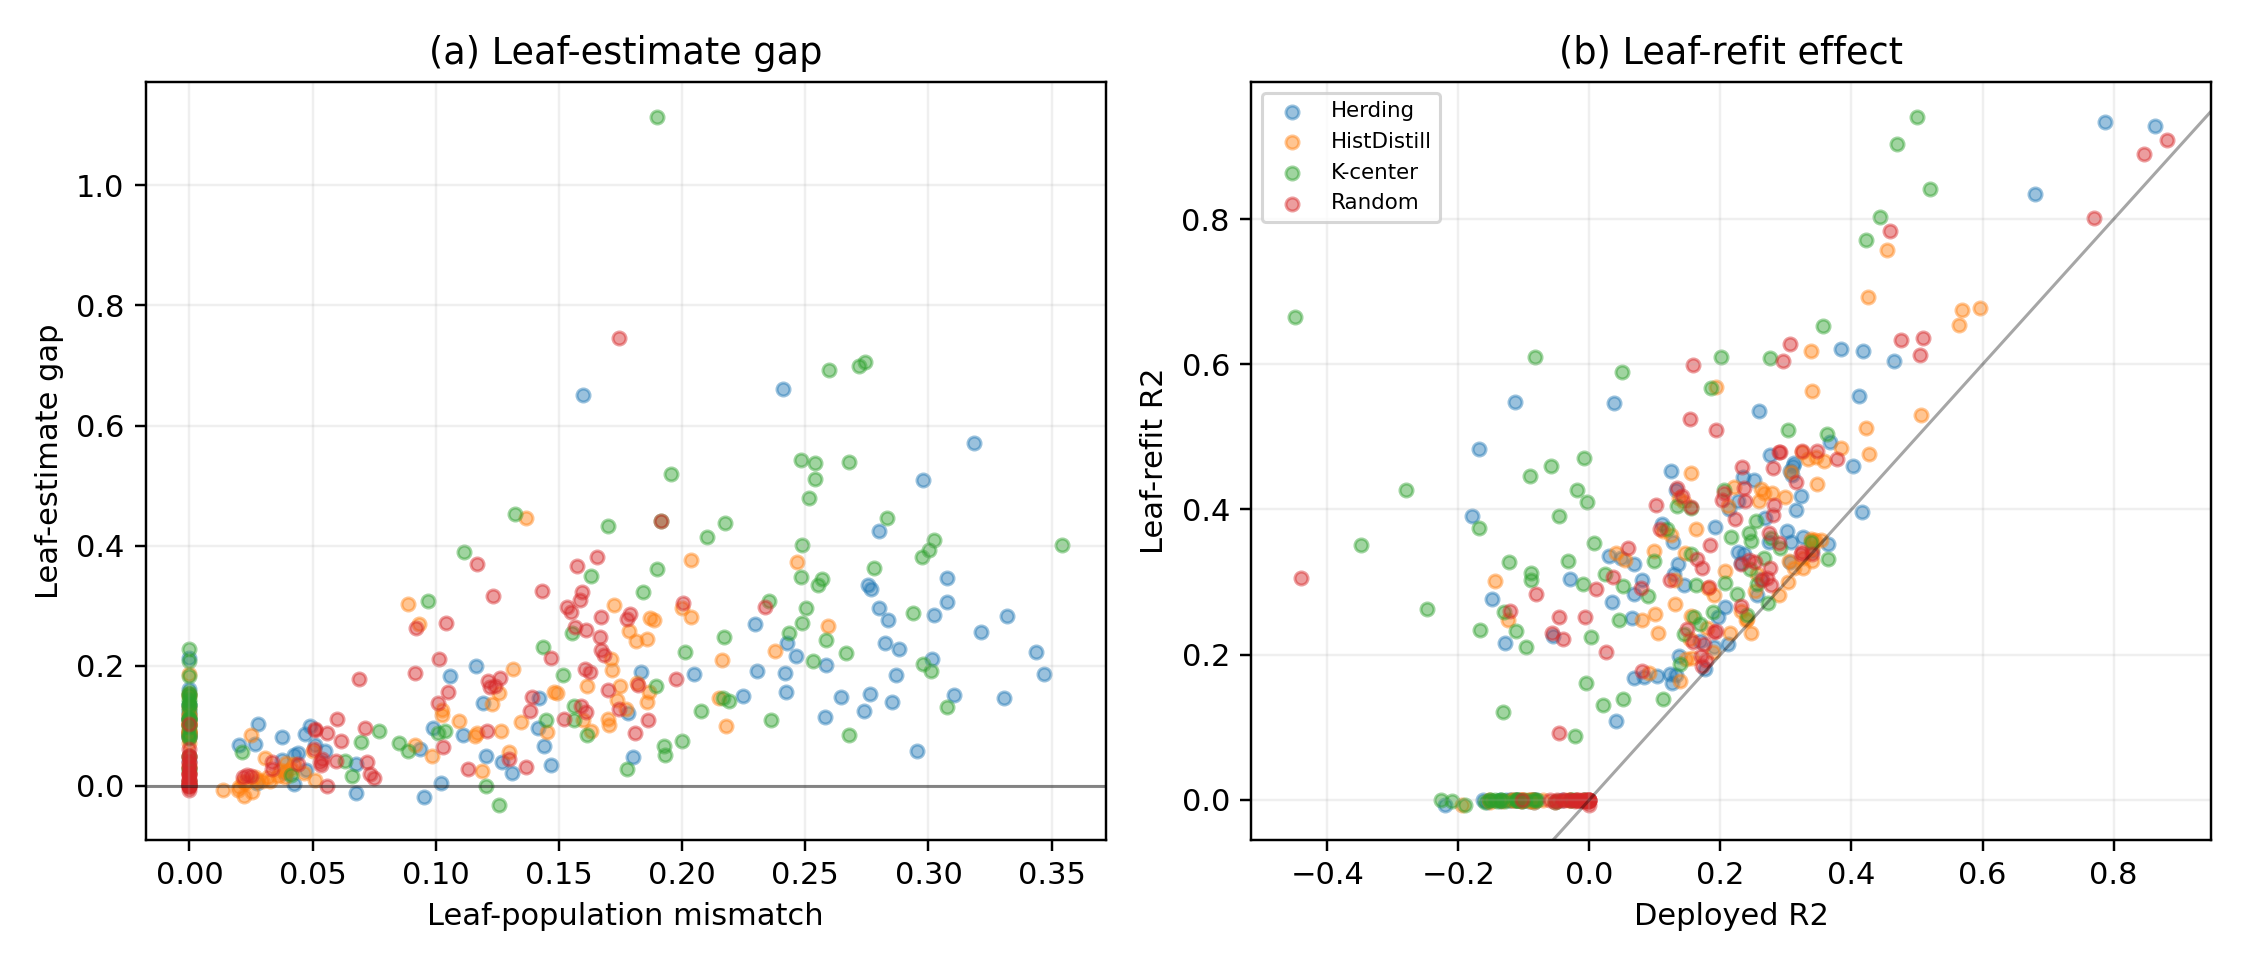
\includegraphics[width=\columnwidth]{figures/phase2_e21_regression_decomposition.png}
\caption{%
  \textbf{Regression decomposition.}
  Structure loss dominates for every method; leaf refitting helps modestly but
  does not close the gap to the structure reference.%
}
\label{fig:regression}
\end{figure}

\textbf{HPO configuration rankings transfer poorly from condensed to full data.}
Across 12 binary datasets, the top-3 agreement between condensed- and full-data
HPO rankings is $4.2\%$ and the top-1 match rate is $8.3\%$, with a
configuration rank correlation near zero ($0.15$). The median retraining
speedup is $1.6\times$, far too small to compensate. Condensed HPO can find a
competitive configuration by chance, but it finds a different one rather than
the full-data optimum. Top configurations selected on a condensed set should
always be validated on full data before deployment.

\textbf{Training-free selection of the single best method is unreliable.}
Split-regret reliably orders method families (Spearman $\rho=-0.87$), but
per-dataset selection of the single best method is harder. The top-3 success
rate of the SLD-based selector is $43.6\%$ and the top-1 rate is $12.2\%$
across all dataset--budget cells. When the second- and third-ranked methods are
close in regret, as is typical, the score is more useful as a rejection filter
for clearly poor surrogates than as an oracle.

Across five multiclass datasets the gain-path family improves over Random by
$1.3\%$ macro-AUROC, a positive but thin extension of the binary results. Taken
together, these findings confirm that SLD is a measurement instrument designed
around the GBDT split-gain objective; its signal erodes wherever that objective
does not govern the learning.
